\documentclass[a4paper,11pt,dvipsnames]{book}
\renewcommand{\familydefault}{\sfdefault}

\usepackage{standalone}
\usepackage[english]{babel}
\usepackage[top=3cm]{geometry}
\usepackage{float}
\usepackage{tabularx}
\usepackage{multirow}
\usepackage{booktabs}
\usepackage{pgfplots}
\usepackage{amsmath}
\usepackage{amssymb}
\usepackage{amsfonts}
\usepackage{siunitx}
\usepackage{tikz}
\usepackage{graphics} % for pdf, bitmapped graphics files
\usepackage{graphicx}
\usepackage{exsheets}
\usepackage{algorithm}
\usepackage{algorithmicx}
\usepackage[noend]{algpseudocode}
\usepackage{hyperref}
\usepackage{enumitem}
\usepackage{filecontents}
\usepackage{multirow}
%\usepackage{showframe}% to show frames
%\ifCLASSOPTIONcompsoc
\usepackage[caption=false, font=normalsize, labelfont=sf, textfont=sf]{subfig}
%\else
%\usepackage[caption=false, font=footnotesize]{subfig}
%\fi    

\usetikzlibrary{patterns,arrows,arrows.meta,calc,intersections,shapes,positioning,decorations.pathreplacing,decorations.markings,decorations.pathmorphing}
\usepackage{multicol}

\sisetup{output-decimal-marker={,},exponent-product=\cdot}

\DeclareSIUnit\atm{atm}
\DeclareSIUnit\dioptre{D}



\def\BState{\State\hskip-\ALG@thistlm}


\definecolor{TitleColor}{rgb}{0.65,0.04,0.07}
\definecolor{NumberColor}{rgb}{0.02,0.04,0.48}

\DeclareInstance{exsheets-heading}{fancy}{default}{
toc-reversed = true ,
indent-first = true ,
vscale = 2 ,
pre-code = \IfInsideQuestionT{\rule{\linewidth}{1pt}} ,
post-code =\IfInsideQuestionT{\rule{\linewidth}{1pt}} ,
subtitle-format = \large\scshape\color{rgb:red,0.65;green,0.04;blue,0.07} ,
number-format = \large\bfseries\color{rgb:red,0.02;green,0.04;blue,0.48} ,
points-format = \itshape ,
join = { number[r,B]title[l,B](.333em,0pt);
title[r,B]subtitle[l,B](1em,0pt)
} ,
attach =
{
main[hc,vc]number[hc,vc](0pt,0pt) ;
main[l,vc]subtitle[hc,vc](\marginparsep,0pt)
}
}



\DeclareInstance{exsheets-heading}{block-subtitle}{default}{
vscale = 2 ,
pre-code = \rule{\linewidth}{1pt} ,
post-code = \rule{\linewidth}{1pt} ,%title-format = \large\scshape\color{TitleColor} ,
number-format = \large\bfseries\color{rgb:red,0.02;green,0.04;blue,0.48} ,
subtitle-format = \large\scshape\color{black} ,
join = {
title[r,B]number[l,B](.333em,0pt) ;
title[r,B]subtitle[l,B](1em,0pt)
} ,
attach = {
main[l,vc]title[l,vc](0pt,0pt) ;
main[r,vc]points[l,vc](\marginparsep,0pt)
},
}

\DeclareQuestionClass{textbook}{textbooks}

\SetupExSheets{
  headings = fancy,
  question/print = true ,
  solution/print = false }
 % counter-format = se.qu ,
%  counter-within = section ,
  %question/pre-hook = \rule{\textwidth}{1pt},


\hypersetup{
	colorlinks = true, 
	breaklinks = true, 
	bookmarks = true,
	bookmarksnumbered = true,
	urlcolor = blue, 
	linkcolor = blue, 
	citecolor=blue,
	linktoc=page, 
	pdftitle={}, 
	pdfauthor={\textcopyright Author}, 
	pdfsubject={}, 
	pdfkeywords={}, 
	pdfcreator={pdfLaTeX}, % PDF Creator
	pdfproducer={IEEE} }





\tikzset{point/.style={circle,fill,black!80,inner sep=0pt,minimum size=#1,opacity=0.9}}
\tikzset{point/.default=3pt}\tikzset{vector/.style={line width=1pt,postaction={decorate,decoration={markings,mark=at position 1 with {\arrow{latex}}}}}}
\tikzset{block/.style={rectangle,fill=black!30,draw,minimum size=#1,opacity=0.9,align=center}}
\tikzset{block/.default=15pt}\tikzset{ball/.style={circle,fill=black!30,draw,minimum size=#1,opacity=0.9}}
\tikzset{ball/.default=5pt}\tikzset{pulley/.style={draw=black,line width=0.2pt,circle,minimum size=#1,inner sep=0pt,fill=black!10}}
\tikzset{pulley/.default=20pt}\tikzset{rod/.style={line width=2pt}}
\tikzset{rope/.style={line width=1pt}}
\tikzset{spring/.style={decorate,decoration={coil,amplitude=5pt,segment length=#1,aspect=0.3}}}
\tikzset{spring/.default=5pt}\tikzset{wall/.style={black!10,pattern=north east lines,opacity=0.3}}
\tikzset{ray/.style={line width=0.8pt,postaction={decorate,decoration={markings,mark=at position 0.5 with {\arrow{>}}}}}}
\tikzset{arrow/.style={-latex}}
\tikzset{object/.style={line width=1pt,orange,-latex}}
\tikzset{image/.style={line width=1pt,blue,-latex}}
\tikzset{doublearrow/.style={<->,>=latex,thick}}
\tikzset{brace/.style={decorate,decoration={brace,amplitude=#1}}}
\tikzset{brace/.default=5pt}




\graphicspath{{images/}} 




\makeatletter
\@addtoreset{question}{section}
\makeatother


\begin{document}
\author{Dr. Muhammed Rushdi \and Asem Alaa}

\title{Measurements and Instrumentation [SBE206A] (Fall 2018)\\ Midterm Answers}

\maketitle


\chapter*{Question 1: Instrument Types}



\begin{question}

\begin{figure*}[h!]
\centering
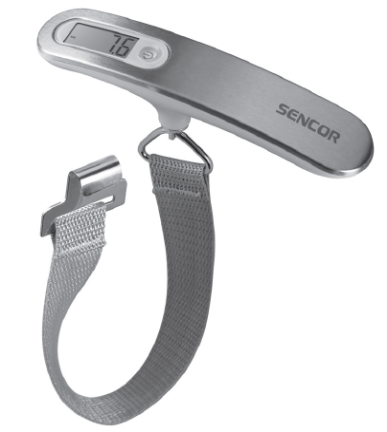
\includegraphics[width=0.3\linewidth]{scale} 
\caption{•}
\end{figure*}

opposite and below figures show a digital travel luggage scale and its technical specifications. Assume the scale has a quoted inaccuracy of $\pm 1\%$ of the full-scale reading. The scale operates as follows:
\begin{enumerate}
\item Pull the nylon strap through the handle of the luggage that you wish to weigh.
\item Hook the buckle of the strap into the triangular loop.
\item Press the power button on the scale. The display will show „8888” and the selected weight measuring unit. 
\item After about two second the scale will be ready for weighing („0.0” will be shown on the display).
\item Now carefully lift the scale together with the luggage in such a way that no part of the luggage is touching the ground or the mat that it is on.
\item After measuring the weight of the weighed item, the measuring unit will flash twice and remain on the display for 30 seconds so that you have enough time to record the weight.
\item Turn off the scale by holding down the power button for 3 seconds. 
\end{enumerate}
{\centering
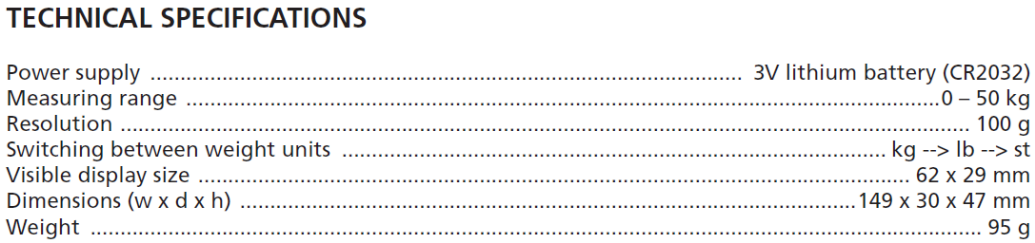
\includegraphics[width=0.8\linewidth]{q1} 
}

Answer the following: 
\begin{enumerate}
\item Specify with justifications whether this instrument is a passive or active instrument, 
\item a deflection-type or null-type instrument, and 
\item an analog or digital instrument. 
\item Comment on the accuracy and ease of use of this instrument. 
\item Can the scale detect a change of 50 g, 95 g, or 149 g? Justify your answers.
\item What is the maximum measurement error expected for this instrument?
\item What is the likely measurement error expressed as a percentage of the output reading if the scale is measuring a weight of 20 kg?
\end{enumerate}



\end{question}
\begin{solution}
\begin{enumerate}
\item Active.
\item Deflection.
\item Digital.
\item (Depends on your previous answers).
\item Can detect 149 g, since it is greater than the instrument resolution.
\item 0.5 Kg.
\item 2.5\%.
\end{enumerate}
\end{solution}


\chapter*{Question 2: Static Characteristics of Instruments}

\begin{question}
A load cell is a sensor used to measure weight. A calibration record table is given below. Determine the maximum error (as a percentage of the full-scale output $y_{\text{FSO}}$ ) for:
 \begin{enumerate}
 \item accuracy $\varepsilon_a = \frac{y_{\text{measured}} - y_{\text{true}}}{y_{\text{FSO}}} \times 100\%$
\item hysteresis $\varepsilon_h = \frac{y_{\text{decreasing}} - y_{\text{increasing}}}{y_{\text{FSO}}} \times 100\%$ 
\item linearity $\varepsilon_l = \frac{y_{\text{measured}} - y_{\text{L}}}{y_{\text{FSO}}} \times 100\%$
\end{enumerate}  
The equation of the best-fit line is $y_L(x) = a_0 + a_1x$, where $a_1=\frac{n\Sigma xy - \Sigma x \Sigma y}{n\Sigma x^2 - {\Sigma x}^2}$, $a_0 = \frac{1}{n}( \Sigma y - a_1 \Sigma x )$, $n$ is the number of data points. Assume that the true or expected output has a linear relationship with the input. In addition, the expected outputs are 0 mV at 0 kg load and 20 mV at 50 kg load. \\
{\centering
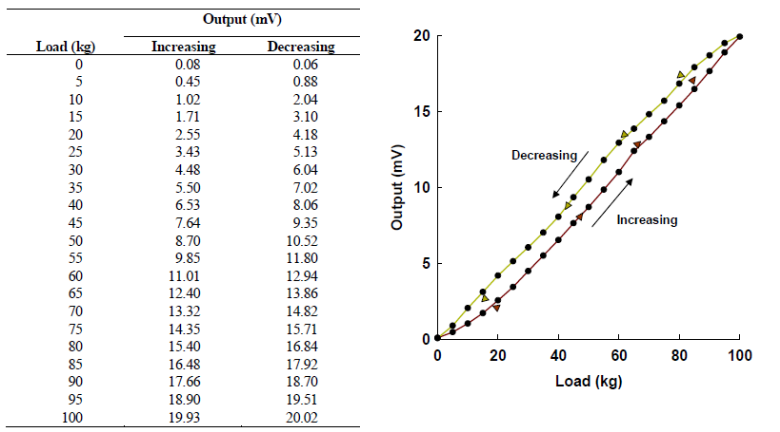
\includegraphics[width=\linewidth]{q2} 
}
\end{question}
\begin{solution}
\begin{enumerate}
\item Maximum difference between the measured and true values occurs at point (25,3.43), hence $\varepsilon_a = \frac{3.43-5}{20} = 7.85\%$
\item Maximum difference between the increasing and decreasing pairs occurs at point load 55 Kg, hence $\varepsilon_h = \frac{11.8-9.85}{20} = 9.75\%$
\item 
Using the calculator (e.g \emph{CASIO fx-570ES PLUS}) on the mode \emph{STAT}: simply issue the \emph{MODE+3}, then select the linear regression model $\rm 2:~ A+BX$; we obtain the following computed parameters: \\
\begin{tabular}{|cc|}
 \hline 
 n  & 42 \\ 
 $\Sigma x$ & 2100 \\ 
 $\Sigma y$ & 409.89 \\ 
 $\Sigma x^2$ & 143500 \\ 
 $\Sigma xy$ & 28499.45 \\ 
 \hline 
 \end{tabular}  \\
 Accordingly, we compute $a_1$ and $a_0$ to get $y_L(x)$ as:\\
 $y_L(x) = -0.6367 + 0.20792 x$ \\
 The maximum difference between the measured and the fitted values, occurs at
 load 40 Kg, hence  $\varepsilon_l = \frac{7.68-6.53}{20} = 5.75\%$
\end{enumerate}
\end{solution}

\chapter*{Question 3: First-Order Instruments}

\begin{question}
A thermocouple is immersed in a liquid to monitor its temperature fluctuations. Assume the thermocouple acts as a first-order system.
\begin{enumerate}
\item In a planned experiment, the thermocouple is to be exposed to a step change in temperature. The
response characteristics of the thermocouple must be such that the thermocouple’s output reaches 95\% of the final temperature within 5 seconds. Assume that the thermocouple’s bead (its sensing element) is spherical with  a density ${\rm \rho = 9000 ~Kg/m^3}$, a specific heat at constant volume ${\rm C_v = 380 ~J/(Kg.K)}$ and a convective heat transfer coefficient $h = 210 ~W/(m^2 K)$. The time constant of the thermocouple is related to those parameters by $\uptau = \frac{\rm \rho d C_v}{6h}$, where $d$ is the diameter of the thermocouple's bead. Determine the \emph{maximum} diameter that the
thermocouple can have and still meet the desired response characteristics.
\item In another experiment on the same thermocouple, the temperature fluctuations (in ${}^\circ C$) vary in time as $T(t) = 30 + 25\cos(4t) + 15\sin(2t)$. The output of the thermocouple transducer system $E(t)$ (in mV) is linearly proportional to temperature and has a static sensitivity of $2~ mV/{}^\circ C$. Find the output $E(t)$ (in mV).
\end{enumerate}
\end{question}

\begin{solution}
\begin{enumerate}
\item  \begin{align*}
0.95 &= 1 - e^{\frac{-5}{\uptau}} \\
\uptau &= \frac{-5}{\ln(0.05)} \\
&= 1.669 s \\
\end{align*} \\
\begin{align*}
1.669 &= \frac{\rm 9000 \times d  \times 380 }{6 \times 210 } \\
d &= 6.15 \times 10^{-4} \\
&= 0.615 mm
\end{align*}
\item By solving the system using Laplace transforms: \\
\begin{align*}
Q_o(s) &= \frac{ K Q_i(s) + \uptau q_o(0) }{ \uptau s + 1} \\
\intertext{Subst. $K=2$, $q_o(0)=0$, $\uptau = 1.67$} 
Q_o(s) &= \frac{ 2Q_i(s) }{ 1.67 s + 1} \\
\because Q_i(s) &= \frac{30}{s} + \frac{25s}{s^2+16} + \frac{30}{s^2+4} \\
\therefore Q_o(s) &= \frac{ \frac{60}{s} + \frac{50s}{s^2+16} + \frac{60}{s^2+4} }{ 1.67 s + 1} \\
&= \frac{110s^4+60s^3+ 1250s^2+960s+3840}{s(1.67s+1)(s^2+16)(s^2+4)} \\
\intertext{Using partial fraction decomposition:}
&= \frac{A}{s} + \frac{B}{1.67s+1} + \frac{Cs+D}{s^2+16} + \frac{Es+F}{s^2+4} \stepcounter{equation}\tag{\theequation}\label{formula1} 
\end{align*}
Marking notes:
\begin{itemize}
\item Obtaining the Equation \eqref{formula1} secures you 9/12 points of this part.
\item Further computation of the constants secures you the full mark.
\item Other solutions of DEs definetly apply. 
\end{itemize}
\end{enumerate}

\end{solution}


\chapter*{Question 4: Second-Order Instruments}

\begin{figure*}[h!]
\centering
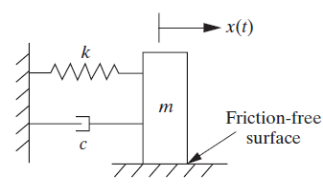
\includegraphics[width=0.3\linewidth]{q4a} 
\caption{•}
\end{figure*}

\begin{figure*}[h!]
\centering
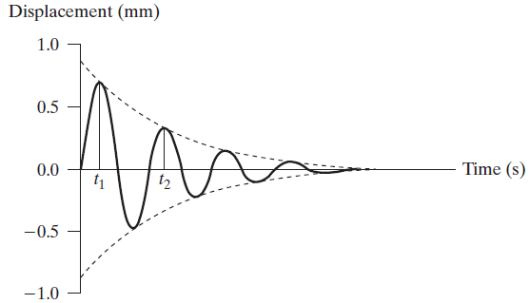
\includegraphics[width=0.5\linewidth]{q4b} 
\caption{•}
\end{figure*}

\begin{question}
The free (natural) response of a second-order measurement instrument that can be modeled as a mass-spring-damper system in Figure 4 (a) with a mass of 2 kg is recorded to be of the form given in Figure 4 (b). A static deflection test is performed and the stiffness is determined to be $k = 1.5 \times 10^3 {\rm N/m}$.
\begin{enumerate}
\item Using the displacements at $t_1$ and $t_2$, calculate the damping coefficient $c$.
\item  Suggest two ways to make the instrument critically damped.
\end{enumerate} 

\end{question}
\begin{solution}
\begin{enumerate}
\item 
\begin{align*}
\omega_n &= \sqrt{\frac{1500}{2}} \\
&= 27.38 {\rm rad/s} \\
\frac{D(t_1)}{D(t_2)} &= e^{\alpha \Delta T} \\ 
\intertext{from graph:}
\frac{0.75}{0.25} &= e^{\alpha \Delta T} \\
\intertext{applying ln on both sides:}
1.1 &= \alpha \Delta T \\ 
\alpha &= 1.1 f_d \\
&= \frac{1.1\omega_d}{2\pi} \\
\because \omega_n^2 &= \omega_d^2 + \alpha^2 \\
&= \omega_d^2 + (\frac{1.1}{2\pi})^2w_d^2 \\
\omega_n &= \omega_d \sqrt{ 1 + (\frac{1.1}{2\pi})^2 } \\
\therefore \omega_n &= 1.02 \omega_d \\
\therefore \sqrt{1-\zeta^2} &= 1/1.02 = 0.98  \\
\zeta &= 0.2 \\
\because \zeta &= \frac{c}{\sqrt{km}} \\
\therefore c = 11 ~{\rm N \cdot Kg / m}
\end{align*}
\item  We manipulate $\zeta$ in order to equal 1, by either:
\begin{enumerate}
\item increasing the damping coeifficient c, or
\item decreasing the spring constant.
\end{enumerate}
\end{enumerate} 
\end{solution}

\begin{question}
State weather the following statements are true or false and correct the false ones:
\begin{enumerate}
\item  Measurement sensitivity describes the closeness of output readings when the same input is applied repetitively over a short period of time, with the same measurement conditions.
\item  Measurement threshold describes the maximum deviation of a manufactured component from some specified value.
\item A measurement system designer should aim to maximize both of the measurement sensitivity and sensitivity to disturbance.
\item The zero drift of an instrument is a lower limit on the magnitude of the change in the input measured quantity that produces an observable change in the instrument output.
\item The sensitivity drift of an instrument describes the effect where the zero reading of an instrument is modified by a change in ambient conditions.
\item Measurement span is defined as the range of different input values over which there is no change in output value.
\item Null-type and deflection-type instruments require two and three inputs, respectively.
\item Passive instruments have higher resolution than active instruments.
\item  The time constant of a first-order instrument is smaller than its half-life time.
\item  For an underdamped second-order instrument, the rise time and settling time are equal.
\end{enumerate}
\end{question}
\begin{solution}
\begin{enumerate}
\item False
\item False
\item True
\item False
\item False
\item False
\item False
\item False
\item False
\item False
\end{enumerate}

\end{solution}

\end{document}
